\section{Cálculo de la Priorización}

\par En este apartado se muestra una comparativa entre el esfuerzo estimado para cada uno de los productos generados en el proyecto y el esfuerzo real dedicado a los mismos. Para ello, se han utilizado las estimaciones realizadas en la planificación y en el documento de cálculo de costes y se han comparado con las hojas de imputación de horas, en las que aparecen las horas reales dedicadas por cada persona a cada uno de los productos.

\subsection{Personal}

\textbf{Alberto García Hernández}
\begin{itemize}
\item Horas respecto al total del proyecto
\end{itemize}
\begin{table}[H]
\begin{center}
\begin{tabular}{ l l l l }
	Actividad & Horas previstas & Horas Reales & Desviación \\ \hline \hline
	 OFE	&	34,44	&	27,35	&	7,09	\\ \hline
DCC	&	34,44	&	33,56	&	0,88	\\ \hline
EVS	&	114,82	&	128,74	&	-13,92	\\ \hline
IQS1	&	11,48	&	12,3	&	-0,82	\\ \hline
PGCal	&	43,24	&	44,15	&	-0,90	\\ \hline
GConf	&	43,24	&	44,15	&	-0,90	\\ \hline
PER	&	60,54	&	61,80	&	-1,26	\\ \hline
DAS	&	77,84	&	70,63	&	7,21	\\ \hline
DDS	&	34,60	&	35,32	&	-0,72	\\ \hline
IQS2	&	17,30	&	8,83	&	8,47	\\ \hline
\end{tabular}
\caption{Alberto:Horas respecto al total del proyecto.}
\label{tab:Alberto:HorasTotalInforme_2}
\end{center}
\end{table}

\begin{itemize}
\item Horas respecto al total del proyecto
\end{itemize}
\begin{table}[H]
\begin{center}
\begin{tabular}{ l l l l l }
	 Actividad & Horas previstas & Horas Reales & Desviación \\ \hline \hline

PGCal	&	43,24	&	44,15	&	-0,90	\\ \hline
GConf	&	43,24	&	44,15	&	-0,90	\\ \hline
PER	&	60,54	&	61,80	&	-1,26	\\ \hline
DAS	&	77,84	&	70,63	&	7,21	\\ \hline
DDS	&	34,60	&	35,32	&	-0,72	\\ \hline
IQS2	&	17,30	&	8,83	&	8,47	\\ \hline
\end{tabular}
\caption{Alberto:Periodo contemplado en este informe.}
\label{tab:Alberto:PeriodoContempladoInforme_2}
\end{center}
\end{table}

\newpage

\textbf{Juan Abascal Sánchez}
\begin{itemize}
\item Horas respecto al total del proyecto
\end{itemize}
\begin{table}[H]
\begin{center}
\begin{tabular}{ l l l l }
  Actividad & Horas previstas & Horas Reales & Desviación \\ \hline \hline
OFE	&	23,76	&	18,65	&	5,11	\\ \hline
DCC	&	23,76	&	22,93	&	0,83	\\ \hline
EVS	&	79,22	&	87,32	&	-8,1	\\ \hline
IQS1	&	7,92	&	6,49	&	1,43	\\ \hline
PGCal	&	30,61	&	31,25	&	-0,64	\\ \hline
GConf	&	30,61	&	31,25	&	-0,64	\\ \hline
PER	&	42,86	&	43,75	&	-0,89	\\ \hline
DAS	&	55,10	&	50,00	&	5,10	\\ \hline
DDS	&	24,49	&	25,00	&	-0,51	\\ \hline
IQS2	&	12,24	&	6,25	&	5,99	\\ \hline
\end{tabular}
\caption{Juan:Horas respecto al total del proyecto.}
\label{tab:Juan:HorasTotalInforme_2}
\end{center}
\end{table}

\begin{itemize}
\item Horas respecto al total del proyecto
\end{itemize}
\begin{table}[H]
\begin{center}
\begin{tabular}{ l l l l l }
  Actividad & Horas previstas & Horas Reales & Desviación \\ \hline \hline
PGCal	&	30,61	&	31,25	&	-0,64	\\ \hline
GConf	&	30,61	&	31,25	&	-0,64	\\ \hline
PER	&	42,86	&	43,75	&	-0,89	\\ \hline
DAS	&	55,10	&	50,00	&	5,10	\\ \hline
DDS	&	24,49	&	25,00	&	-0,51	\\ \hline
IQS2	&	12,24	&	6,25	&	5,99	\\ \hline
\end{tabular}
\caption{Juan:Periodo contemplado en este informe.}
\label{tab:Juan:PeriodoContempladoInforme_2}
\end{center}
\end{table}

\newpage


\textbf{Daniel González de la Hera}
\begin{itemize}
\item Horas respecto al total del proyecto
\end{itemize}
\begin{table}[H]
\begin{center}
\begin{tabular}{ l l l l }
  Actividad & Horas previstas & Horas Reales & Desviación \\ \hline \hline
OFE	&	3,1	&	2,97	&	0,13	\\ \hline
DCC	&	3,1	&	3,13	&	-0,03	\\ \hline
EVS	&	10,33	&	18,03	&	-7,7	\\ \hline
IQS1	&	1,33	&	1,28	&	0,05	\\ \hline
PGCal	&	12,24	&	12,50	&	-0,26	\\ \hline
GConf	&	12,24	&	12,50	&	-0,26	\\ \hline
PER	&	17,14	&	17,50	&	-0,36	\\ \hline
DAS	&	22,04	&	20,00	&	2,04	\\ \hline
DDS	&	9,80	&	10,00	&	-0,20	\\ \hline
IQS2	&	4,90	&	2,50	&	2,40	\\ \hline
\end{tabular}
\caption{Daniel:Horas respecto al total del proyecto.}
\label{tab:Daniel:HorasTotalInforme_2}
\end{center}
\end{table}

\begin{itemize}
\item Horas respecto al total del proyecto
\end{itemize}
\begin{table}[H]
\begin{center}
\begin{tabular}{ l l l l l }
  Actividad & Horas previstas & Horas Reales & Desviación \\ \hline \hline
PGCal	&	12,24	&	12,50	&	-0,26	\\ \hline
GConf	&	12,24	&	12,50	&	-0,26	\\ \hline
PER	&	17,14	&	17,50	&	-0,36	\\ \hline
DAS	&	22,04	&	20,00	&	2,04	\\ \hline
DDS	&	9,80	&	10,00	&	-0,20	\\ \hline
IQS2	&	4,90	&	2,50	&	2,40	\\ \hline
\end{tabular}
\caption{Daniel:Periodo contemplado en este informe.}
\label{tab:Daniel:PeriodoContempladoInforme_2}
\end{center}
\end{table}

\newpage


\textbf{Carlos Olivares Sánchez-Manjavacas}
\begin{itemize}
\item Horas respecto al total del proyecto
\end{itemize}
\begin{table}[H]
\begin{center}
\begin{tabular}{ l l l l }
  Actividad & Horas previstas & Horas Reales & Desviación \\ \hline \hline
OFE	&	3,44	&	2,87	&	0,57	\\ \hline
DCC	&	3,44	&	3,34	&	0,1	\\ \hline
EVS	&	11,48	&	19,23	&	-7,75	\\ \hline
IQS1	&	1,14	&	1,18	&	-0,04	\\ \hline
PGCal	&	6,13	&	6,26	&	-0,13	\\ \hline
GConf	&	6,13	&	6,26	&	-0,13	\\ \hline
PER	&	8,59	&	8,76	&	-0,18	\\ \hline
DAS	&	11,04	&	10,02	&	1,02	\\ \hline
DDS	&	4,91	&	5,01	&	-0,10	\\ \hline
IQS2	&	2,45	&	1,25	&	1,20	\\ \hline
\end{tabular}
\caption{CarlosOSM:Horas respecto al total del proyecto.}
\label{tab:CarlosOSM:HorasTotalInforme_2}
\end{center}
\end{table}

\begin{itemize}
\item Horas respecto al total del proyecto
\end{itemize}
\begin{table}[H]
\begin{center}
\begin{tabular}{ l l l l l }
  Actividad & Horas previstas & Horas Reales & Desviación \\ \hline \hline
PGCal	&	6,13	&	6,26	&	-0,13	\\ \hline
GConf	&	6,13	&	6,26	&	-0,13	\\ \hline
PER	&	8,59	&	8,76	&	-0,18	\\ \hline
DAS	&	11,04	&	10,02	&	1,02	\\ \hline
DDS	&	4,91	&	5,01	&	-0,10	\\ \hline
IQS2	&	2,45	&	1,25	&	1,20	\\ \hline
\end{tabular}
\caption{CarlosOSM:Periodo contemplado en este informe.}
\label{tab:CarlosOSM:PeriodoContempladoInforme_2}
\end{center}
\end{table}

\newpage


\textbf{Carlos Tormo Sánchez}
\begin{itemize}
\item Horas respecto al total del proyecto
\end{itemize}
\begin{table}[H]
\begin{center}
\begin{tabular}{ l l l l }
Actividad & Horas previstas & Horas Reales & Desviación \\ \hline \hline
OFE	&	0,34	&	0,26	&	0,08	\\ \hline
DCC	&	0,34	&	0,33	&	0,01	\\ \hline
EVS	&	1,14	&	3,21	&	-2,07	\\ \hline
IQS1	&	0,11	&	0,13	&	-0,02	\\ \hline
PGCal	&	1,05	&	1,08	&	-0,02	\\ \hline
GConf	&	1,05	&	1,08	&	-0,02	\\ \hline
PER	&	1,47	&	1,51	&	-0,03	\\ \hline
DAS	&	1,90	&	1,72	&	0,18	\\ \hline
DDS	&	0,84	&	0,86	&	-0,02	\\ \hline
IQS2	&	0,42	&	0,22	&	0,21	\\ \hline
\end{tabular}
\caption{CarlosTS:Horas respecto al total del proyecto.}
\label{tab:CarlosTS:HorasTotalInforme_2}
\end{center}
\end{table}

\begin{itemize}
\item Horas respecto al total del proyecto
\end{itemize}
\begin{table}[H]
\begin{center}
\begin{tabular}{ l l l l l }
  Actividad & Horas previstas & Horas Reales & Desviación \\ \hline \hline

PGCal	&	1,05	&	1,08	&	-0,02	\\ \hline
GConf	&	1,05	&	1,08	&	-0,02	\\ \hline
PER	&	1,47	&	1,51	&	-0,03	\\ \hline
DAS	&	1,90	&	1,72	&	0,18	\\ \hline
DDS	&	0,84	&	0,86	&	-0,02	\\ \hline
IQS2	&	0,42	&	0,22	&	0,21	\\ \hline
\end{tabular}
\caption{CarlosTS:Periodo contemplado en este informe.}
\label{tab:CarlosTS:PeriodoContempladoInforme_2}
\end{center}
\end{table}


\newpage


\textbf{Adriana Lima}
\begin{itemize}
\item Horas respecto al total del proyecto
\end{itemize}
\begin{table}[H]
\begin{center}
\begin{tabular}{ l l l l }
	Actividad & Horas previstas & Horas Reales & Desviación \\ \hline \hline
OFE	&	3,44	&	2,87	&	0,57	\\ \hline
DCC	&	3,44	&	3,34	&	0,1	\\ \hline
EVS	&	11,48	&	19,23	&	-7,75	\\ \hline
IQS1	&	1,14	&	1,18	&	-0,04	\\ \hline
PGCal	&	6,13	&	6,26	&	-0,13	\\ \hline
GConf	&	6,13	&	6,26	&	-0,13	\\ \hline
PER	&	8,59	&	8,76	&	-0,18	\\ \hline
DAS	&	11,04	&	10,02	&	1,02	\\ \hline
DDS	&	4,91	&	5,01	&	-0,10	\\ \hline
IQS2	&	2,45	&	1,25	&	1,20	\\ \hline
\end{tabular}
\caption{Adriana:Horas respecto al total del proyecto.}
\label{tab:Adriana:HorasTotalInforme_2}
\end{center}
\end{table}

\begin{itemize}
\item Horas respecto al total del proyecto
\end{itemize}
\begin{table}[H]
\begin{center}
\begin{tabular}{ l l l l l }
  Actividad & Horas previstas & Horas Reales & Desviación \\ \hline \hline
PGCal	&	6,13	&	6,26	&	-0,13	\\ \hline
GConf	&	6,13	&	6,26	&	-0,13	\\ \hline
PER	&	8,59	&	8,76	&	-0,18	\\ \hline
DAS	&	11,04	&	10,02	&	1,02	\\ \hline
DDS	&	4,91	&	5,01	&	-0,10	\\ \hline
IQS2	&	2,45	&	1,25	&	1,20	\\ \hline
\end{tabular}
\caption{Adriana:Periodo contemplado en este informe.}
\label{tab:Adriana:PeriodoContempladoInforme_2}
\end{center}
\end{table}


\newpage


\textbf{Irina Shayk}
\begin{itemize}
\item Horas respecto al total del proyecto
\end{itemize}
\begin{table}[H]
\begin{center}
\begin{tabular}{ l l l l }
	Actividad & Horas previstas & Horas Reales & Desviación \\ \hline \hline
OFE	&	0,34	&	0,26	&	0,08	\\ \hline
DCC	&	0,34	&	0,33	&	0,01	\\ \hline
EVS	&	1,14	&	3,21	&	-2,07	\\ \hline
IQS1	&	0,11	&	0,13	&	-0,02	\\ \hline
PGCal	&	1,05	&	1,08	&	-0,02	\\ \hline
GConf	&	1,05	&	1,08	&	-0,02	\\ \hline
PER	&	1,47	&	1,51	&	-0,03	\\ \hline
DAS	&	1,90	&	1,72	&	0,18	\\ \hline
DDS	&	0,84	&	0,86	&	-0,02	\\ \hline
IQS2	&	0,42	&	0,22	&	0,21	\\ \hline
\end{tabular}
\caption{Irina:Horas respecto al total del proyecto.}
\label{tab:Irina:HorasTotalInforme_2}
\end{center}
\end{table}

\begin{itemize}
\item Horas respecto al total del proyecto
\end{itemize}
\begin{table}[H]
\begin{center}
\begin{tabular}{ l l l l l }
  Actividad & Horas previstas & Horas Reales & Desviación \\ \hline \hline
PGCal	&	1,05	&	1,08	&	-0,02	\\ \hline
GConf	&	1,05	&	1,08	&	-0,02	\\ \hline
PER	&	1,47	&	1,51	&	-0,03	\\ \hline
DAS	&	1,90	&	1,72	&	0,18	\\ \hline
DDS	&	0,84	&	0,86	&	-0,02	\\ \hline
IQS2	&	0,42	&	0,22	&	0,21	\\ \hline
\end{tabular}
\caption{Irina:Periodo contemplado en este informe.}
\label{tab:Irina:PeriodoContempladoInforme_2}
\end{center}
\end{table}

\newpage


\subsection{Recursos acumulados}

\begin{table}[h]
\begin{center}
\begin{tabular}{ p{1.75cm}  p{1.25cm}  p{1.25cm} p{1.25cm}  p{1.25cm}  p{1.25cm}  p{1.25cm}  p{1.25cm} p{1.25cm} p{1.25cm}}

	Documento &  Tipo & 06/02/17 & 20/02/17 & 06/03/17 & 20/03/17 & 3/04/17 & 17/04/17 & 01/05/17 & 12/05/17\\ \hline \hline

	OFE & Estimado & 65.10 & 65.10 & 65.10 &  65.10 &  65.10 &  65.10 &  65.10 & 65.10 \\
	 		& Real & 55.42 & 55.42 & 55.42 & 55.42 & 55.42 & 55.42 & 55.42 & 55.42\\ \hline

		DCC & Estimado & 65.10 & 65.10 & 65.10 &  65.10 &  65.10 &  65.10 &  65.10 & 65.10 \\
	 			& Real & 69.05 & 69.05 & 69.05 & 69.05 & 69.05 & 69.05 & 69.05 & 69.05\\ \hline

		EVS & Estimado & 217.01 & 217.01 & 217.01 &  217.01&  217.01&  217.01&  217.01& 217.01\\
				& Real & 0 & 275.19 & 275.19 & 275.19 & 275.19 & 275.19 & 275.19 & 275.19\\ \hline

		IQS1 & Estimado & 21.7 & 21.7 & 21.7 &  21.7&  21.7&  21.7&  21.7& 21.7\\
	 			& Real & 0 & 0 & 22.71 & 22.71 & 22.71 & 22.71 & 22.71 & 22.71\\ \hline

	 PGCal & Estimado & 100.47 &  100.47 &  100.47 &  100.47&  100.47&  100.47&  100.47& 100.47\\
 	 			& Real & 0 & 85.43 & 102.57 &  102.57 &  102.57 &  102.57 &  102.57 & 102.57 \\ \hline

	 GConf & Estimado & 100.47 & 100.47 &  100.47  &  100.47 &  100.47 &  100.47 &  100.47 & 100.47 \\
 	 			& Real & 0 & 0 & 0 &  102.57 &  102.57 &  102.57 &  102.57 & 102.57 \\ \hline

	 PER & Estimado & 140.66 &  140.66  &  140.66  &  140.66 &  140.66 &  140.66 &  140.66 & 140.66 \\
 	 			& Real & 0 & 0 & 0 & 143.59 &  143.59 &  143.59 &  143.59 & 143.59 \\ \hline

	 DAS & Estimado & 180.85 &  180.85  &  180.85  &  180.85 &  180.85 &  180.85 &  180.85 & 180.85 \\
 	 			& Real & 0 & 0 & 0 & 20.43 &  164.11 &  164.11 &  164.11 & 164.11 \\ \hline

	 DDS & Estimado & 80.38 &  80.38  &  80.38  &  80.38 &  80.38 &  80.38 &  80.38 & 80.38 \\
 	 			& Real & 0 & 0 & 0 & 0 &  82.05 &  82.05 &  82.05 & 82.05 \\ \hline

	 IQS2 & Estimado & 40.19 &  40.19  &  40.19  &  40.19 &  40.19 &  40.19 &  40.19 & 40.19 \\
 	 			& Real & 0 & 0 & 0 & 0 & 0 &  20.51 &  20.51 & 20.51 \\ \hline


\end{tabular}
\caption{Recursos acumulados.}
\label{tab:Recursos acumulados_2}
\end{center}
\end{table}
\pagebreak
\begin{itemize}
\item Gráfica de recursos estimados acumulados
\end{itemize}

\begin{figure}[H]
\begin{center}
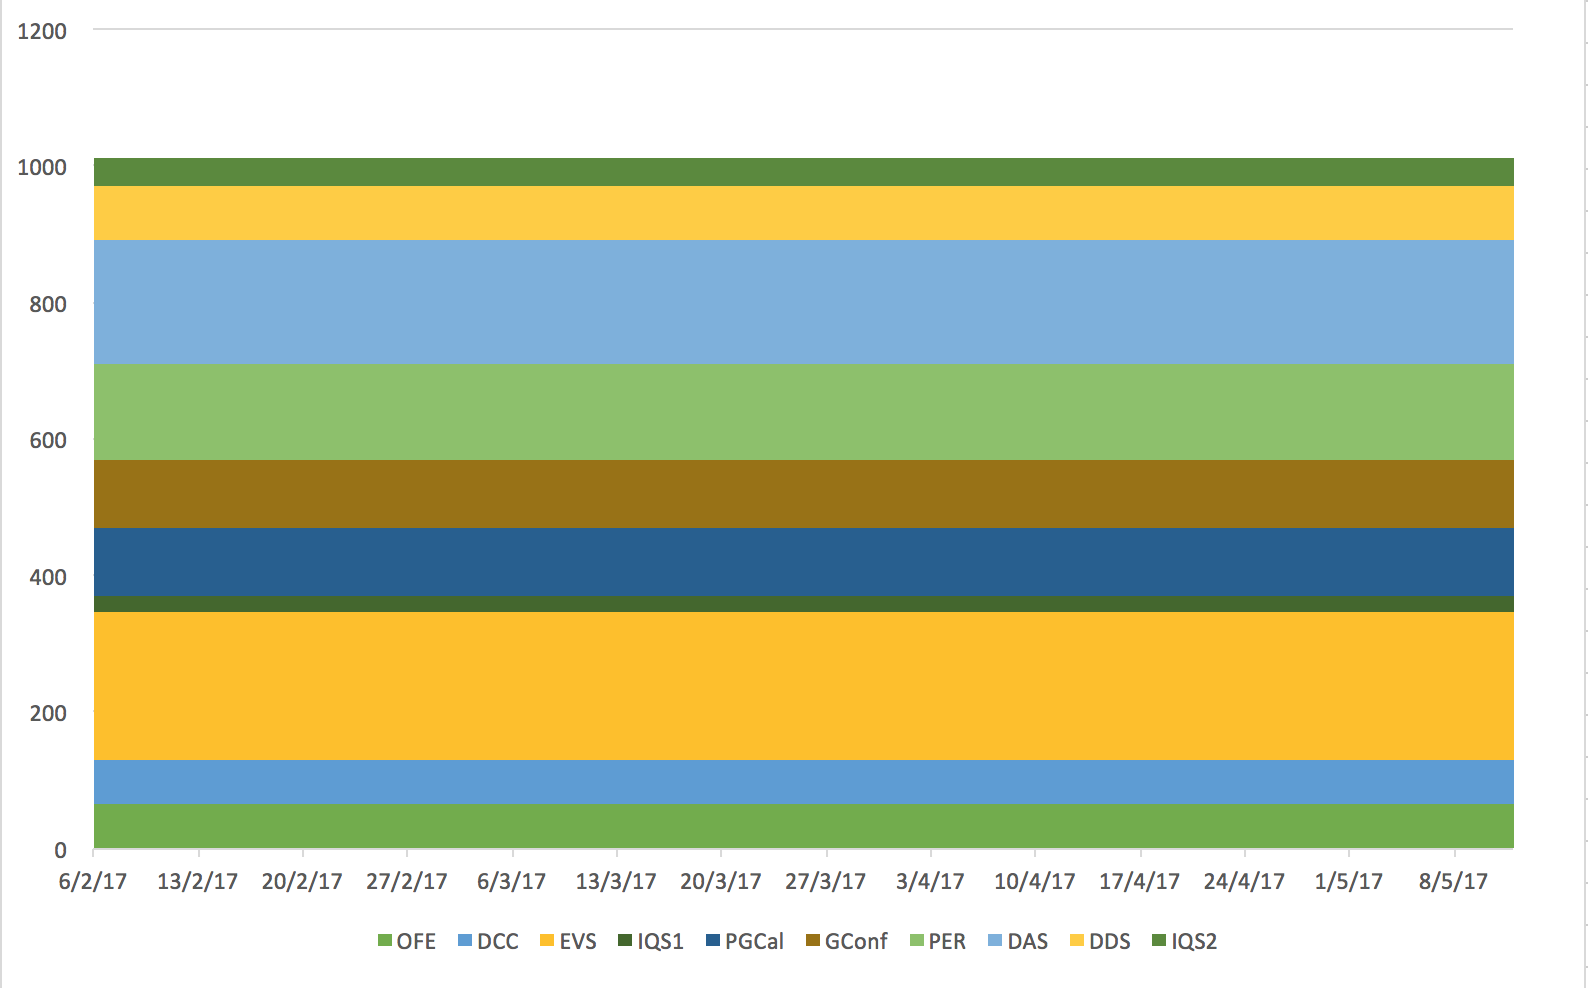
\includegraphics[width=0.8\textwidth]{./img/estimados2.png}
\end{center}
\caption{Gráfica de recursos estimados acumulados}
\label{fig:estimados2}
\end{figure}

\begin{itemize}
\item Gráfica de recursos reales acumulados
\end{itemize}

\begin{figure}[H]
\begin{center}
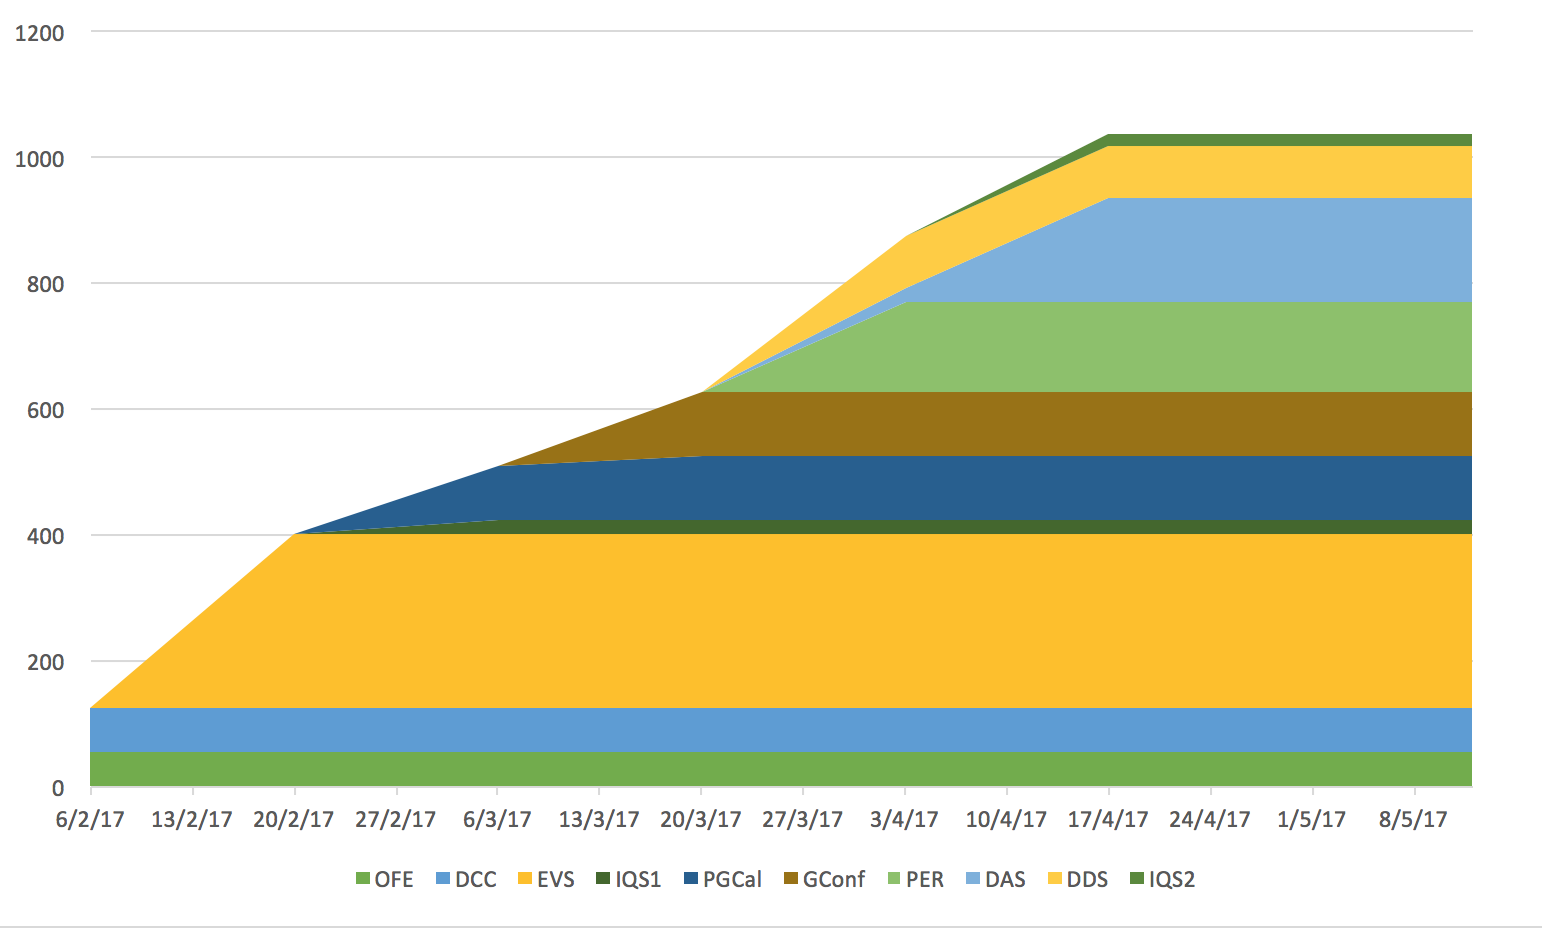
\includegraphics[width=0.8\textwidth]{./img/reales2.png}
\end{center}
\caption{Gráfica de recursos reales acumulados}
\label{fig:reales2}
\end{figure}

\newpage
